%!TEX root = ../report.tex
\documentclass[../report.tex]{subfiles}

\begin{document}
    \section{Methodology}
    \label{sec:methodology}

    % Describe all conceptual details about your approach in this section.
    % Add any necessary subsections to improve the presentation.

    % Feel free to rename this section to better reflect the concrete topic you are discussing.

    % This section details the methodological approach employed to evaluate the efficacy of semantic segmentation models trained on synthetic data generated using AirSim and Unreal Engine. 
    % The evaluation leverages real-world data from the ISPRS dataset and test various hypotheses related to aerial and ground perspectives, data composition, model training strategies, and dataset characteristics. The methodology is organized into the following key components:
    
    % 1. Synthetic Data Generation, 2. Real-World Dataset Selection, 3. Semantic Segmentation Models.
    
    % 1. Synthetic Data Generation: 
    % For the evaluation framerwork first we need to generate the synthetic semantic segmentation to train the models. 
    % a. Tools \& platforms:
    % \subfile{tables/methodology_table1.tex}
    % Hardware requirements:
    % For optimal performance, the following hardware configuration is recommended: 
    % GPU: NVIDIA RTX 3090 with 24 GB VRAM
    % CPU: Intel Core i9-10900K or AMD Ryzen 9 5900X
    % RAM: 128 GB DDR4
    % Storage: 2 TB NVMe SSD
    
    % Environments:
    % Synthetic datasets are created for different aerial heights (10m, 15m, 25m) across various environments, including: City Park, Downtown West, Landscape Mountains Village, Modular Neighborhood package. 

    % AirSim setup: 
    % By following the airsim documentation https://microsoft.github.io/AirSim/ we need to setup unreal project with airsim, it exposes APIs to interact with vehicle in the simulation programmatically using simulated quadrotor, simulated car or computer vision mode.
    
    % Annotations: 
    % Each synthetic image is automatically annotated with precise semantic segmentation masks, ensuring accurate ground truth for model training and evaluation with the help of AirSim Image APIs using computer vision mode.

    % Data Augmentation:
    % Augmentation techniques such as rotation, scaling, and color jittering are applied to enhance dataset variability and robustness.
    
    % We generate the datasets by collecting waypoints in the interested unreal environment's scenes. With those 
    % As part of R\&D we have a data generation pipeline with complete documentation on how to generate the data in the appendix section and also more details can be explored from airsim documentation https://microsoft.github.io/AirSim/. 

    % Once the datasets are generated using our pipeline, we need to choose a real-world dataset for the evaluation of segmentation models. 
    
    % 2. Real-World Dataset: 
    % Aerial real-world datasets are very few in number as manual segmentation of the real-world data is expensive and time consuming. We have choosen ISPRS dataset to compare our results with the real-world data. 

    
    % In this section of the paper the most effective strategies for developing the learning model architecture will be explored. We will also examine the methods and criteria for evaluating its performance, ensuring a comprehensive understanding of both design and assessment processes.

% \begin{figure*}
%   \centering
%   \begin{subfigure}{0.28\linewidth}
%     \includegraphics[width=\textwidth]{figures/binary_threshold.png}
%     \caption{Binary threshold set to 200}
%     \label{fig:binary_threshold}
%   \end{subfigure}
%   \hfill
%   \begin{subfigure}{0.291\linewidth}
%     \includegraphics[width=\textwidth]{figures/set_to_zero.png}
%     \caption{Image set all values below 120 to zero}
%     \label{fig:set_to_zero}
%   \end{subfigure}
%   \hfill
%   \begin{subfigure}{0.305\linewidth}
%     \includegraphics[width=\textwidth]{figures/contrast_stretch.png}
%     \caption{70 \textgreater  Contrast stretch \textless  140}
%     \label{fig:contrast_stretch}
%   \end{subfigure}
%   \caption{Image pre-processing to detect the possible relevant features of a forest ground. Thresholds were selected arbitrarily to enable the clear recognition of particular objects in the image}
%   \label{fig:image_preprocessing}
% \end{figure*}

    This section details the methodological approach employed to evaluate the efficacy of semantic segmentation models trained on synthetic data generated using AirSim and Unreal Engine. 
    We propose 2 staged approaches consisting of 1. Synthetic Data Generation 2. Training and Evaluation of Semantic Segmentation. 
    
    \subsection{Synthetic Data Generation}
    \subsubsection{AirSim Setup}
    To generate the synthetic data, set up Unreal Engine Project(UE versions 4.27+) with AirSim plugin integration using the AirSim repository https://github.com/CodexLabsLLC/Colosseum and follow AirSim documentation https://microsoft.github.io/AirSim/ which exposes APIs to interact with the vehicle in the simulation programmatically using a simulated quadrotor, simulated car or computer vision mode.
    AirSim provides a configuration for users to customize the camera settings to capture the data such as CaptureSettings with ImageType, Width, Height, and FOV\_Degrees, etc which is a key feature for diverse data generation. 
    In order to balance computational demands and preserve visual fidelity, a resolution of 1280x720(720p) standard High Definition (HD) is used. We selected 3 to 4 environments to generate the datasets for our semantic segmentation evaluation with City Park (UE 5.2.1), Downtown West (UE 5.2.1), neighborhood(4.27.2), and Landscape Mountain's Village environment(4.27.2). 
    To achieve optimal segmentation annotations, carefully configured material properties in Unreal Engine (UE) using opaque blend modes and default Lit shading models. To eliminate potential rendering artifacts, we have eliminated post-process volumes from the UE environment.
    
    \subsubsection{Waypoint Collector}
    To reproduce the data collection process, a graphical user interface utilizing PyQt5 is developed to facilitate efficient waypoint collection. Before generating the data, run the UE simulation from the player start position to store the camera coordinates(X, Y, Z) and orientation(W, X, Y, Z) in a JSON format using AirSim's simGetVehiclePose API.
    This system captures camera positions at predefined intervals, maintaining a minimum distance of 0.5 meters between waypoints to ensure comprehensive and diverse scene coverage as showed in the figure. This approach ensures both precision and efficiency in our waypoint collection process for multi-altitudes.

    \begin{figure}
        \centering
        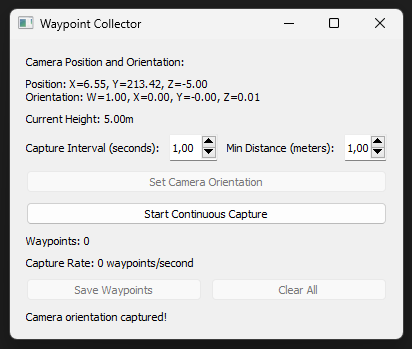
\includegraphics[width=0.5\linewidth]{figures/waypoint_collector.png}
        \caption{Waypoint Collector}
        \label{fig:enter-label}
    \end{figure}
    
    % If material attributes in UE are not set to basic Lit shading models and opaque blend modes the appropriate segmentation would not be assigned.

    \subsubsection{Segmentation Data Generation}
     Our implementation showcases tailored strategies for semantic labeling of desired objects to assign segmentation that effectively addresses the unique challenges posed by different Unreal Engine versions, particularly concerning AirSim integration limitations. In environments built with Unreal Engine 4.27, we developed a label-based mapping approach, primarily due to inconsistencies in how AirSim\'s simListSceneObjects API captures tag-based actors, leading to missing some of the scene objects. This challenge notably impacted InstancedFoliageActors, such as trees and vegetation. To overcome this, we created a label mapping JSON that maps scene objects to their corresponding semantic classes using precise regex patterns. This mapping file is integral to our data generation tool, which adeptly assigns appropriate segmentation IDs to every object in the scene. In contrast, for Unreal Engine 5.2.1 environments, we adopted an efficient tag-based system. Here, objects are strategically tagged with predefined classes like building, road, and tree within the Unreal Editor. We then leverage a custom object extractor script executed within the Unreal Engine framework to comprehensively collect all tagged objects. This script generates a JSON file that outlines each object's structured list and its respective tags. Our data generation tool uses this JSON file to assign segmentation IDs to objects utilizing AirSim\'s simSetSegmentationObjectID API. Both approaches adhere to a unified segmentation color scheme of RGB format "https://github.com/microsoft/AirSim/blob/main/docs/seg_rgbs.txt", with buildings [196, 30, 8], roads [102, 16, 239], trees [11, 236, 9], vegetation [153, 108, 6], vehicles [242, 107, 146], humans [255, 255, 255], and clutter [0, 0, 0]. Prior to assigning new segmentation IDs, our system rigorously resets all existing IDs to 0, ensuring pristine segmentation masks. This dual methodology not only guarantees consistent semantic labeling across various Unreal Engine versions but also enriches the quality and reliability of the generated segmentation masks. 

     \begin{figure}
        \centering
        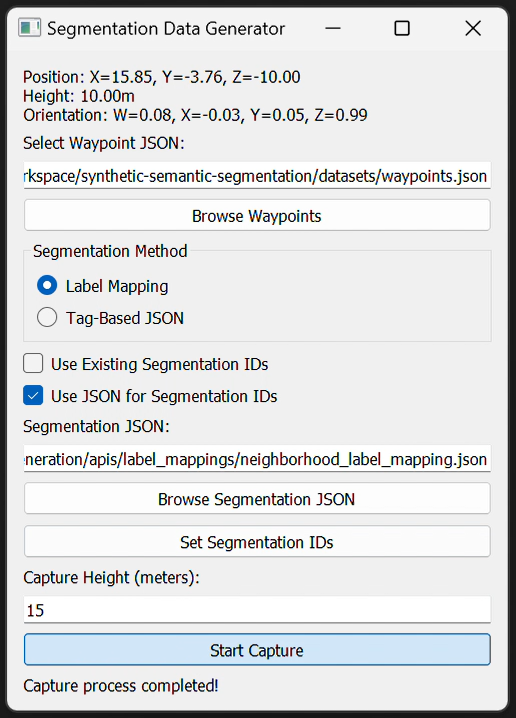
\includegraphics[width=0.5\linewidth]{figures/segmentation_data_generator.png}
        \caption{Waypoint Collector}
        \label{fig:enter-label}
    \end{figure}
    
     Waypoints collected from the waypoint collector tool are used in the segmentation data generator tool, by specifying the required capture height with the North-East-Down (NED) coordinate system, which utilizes camera height as a negative Z-coordinate. The collected data is categorized and stored into height-specific directories, such as "10m," "15m," or "25m". Additionally, logs the comprehensive metadata for each collection, which includes key height and capture parameters, ensuring robust data provenance. This approach guarantees consistent and reproducible data collection across various altitudes, crucial for analyzing the impact of height on segmentation performance and developing effective segmentation models at different flying heights.

     Time Analysis of data generation in our approach is observed that capturing each waypoint with the collection tool typically requires around 1 second. Following this, the data generation process encompassing camera positioning, RGB, and segmentation mask capture, verification, and storage averages about 3 seconds per image pair. Our implementation results revealed that capturing 34 image pairs was accomplished in 99.58 seconds without any quality issues or failed captures. Based on this performance, we can anticipate that generating a dataset of 1000 image pairs would require approximately less than an hour dedicated solely to the data generation phase.

    \subsection{Training and Evaluation Framework}
    The training strategies are followed from the paper "UAVid: A Semantic Segmentation Dataset for UAV Imagery" \cite{lyu2020uavid}
    The generated synthetic dataset is systematically organized into train, validation, and test splits, adhering to the author Lyu's strategic ratio of 3:1:2. Each split comprises paired RGB images alongside their corresponding segmentation masks, captured at specified altitudes of 10m, 15m, and 25m. Datasets collected from multiple environments are combined to train and evaluate against real dataset. 

    \subsubsection{Model Architecture and Training}
    Our framework employs two semantic segmentation architectures: UNet with a ResNet34 backbone an encoder-decoder architecture and a transformer architecture, SegFormer-B3, both recognized for their exceptional performance in segmentation tasks. The implementation of UNet is facilitated by the established segmentation models library from PyTorch(https://smp.readthedocs.io/en/latest/models.html#unet), while the SegFormer model is integrated using the HuggingFace model(https://huggingface.co/nvidia/segformer-b3-finetuned-cityscapes-1024-1024). 
    Both architectures receive input images of size 512×512, standardized through resizing and normalization using mean(0.485, 0.456, 0.406) and standard deviation(0.229, 0.224, 0.225) to match the ImageNet pre-training statistics. We apply data augmentation for train split such as left-to-right flip randomly, color augmentation, including random hue operation, random contrast operation, random brightness operation, random saturation operation.
    For real-world datasets, an additional color mapping mechanism ensures consistency between synthetic and real data by converting real-world mask colors to match the synthetic labels for visualization of predictions during evaluation.
    
    % The training pipeline is comprehensively designed and includes: - A custom dataset class that effectively manages both synthetic and real data. - Innovative data augmentation techniques applied through the albumentations library, which significantly enhance model generalization and enable robust performance across various conditions. 
    Custom dataset class handling both synthetic and real data 
    Data augmentation using albumentations library for improved generalization 
    Learning rate scheduling with exponential decay 
    Regular model checkpointing and performance logging 

    
\end{document}

